%\todo{Make sure that all $k$-space functions have tildes.  Or not, but be consistent with other chapters.}
\begin{figure}[ht]
 \centering
 \import{includes/}{setpgfinc}
 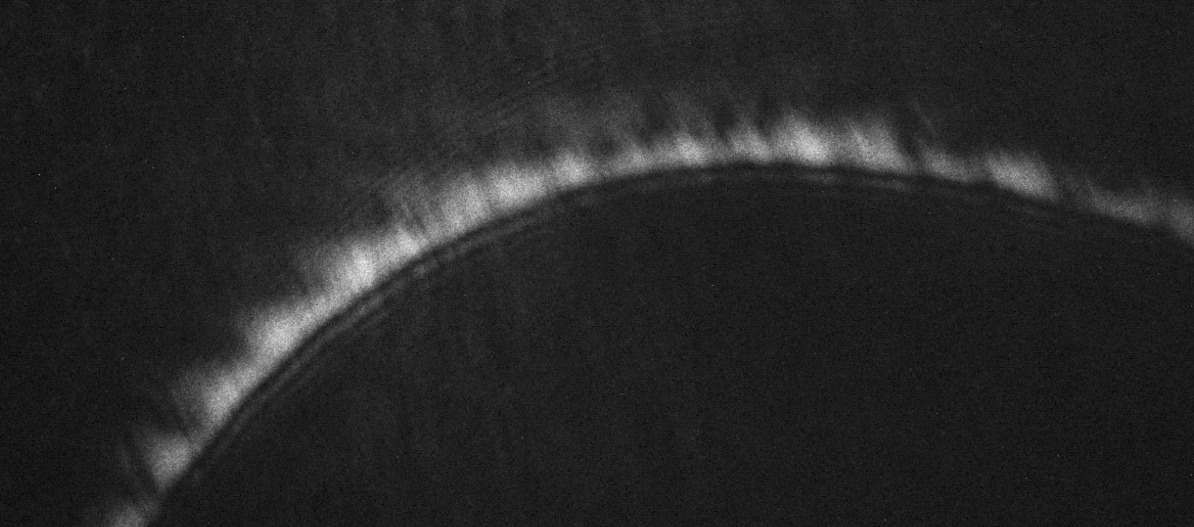
\includegraphics[keepaspectratio,width=15.5cm]{interference/figures/coneintro.png}
 \caption{Section of the cone exhibiting one sided interference fringes.
 System parameters: $\lambda_0 = \SI{632.8}{\nano\meter}$,
 $n_1=1.9961$ (LAH79), $n_2 = \num{-14.48+1.09i}$ (silver), $n_3=1.0$
 (air), and $d_2=\SI{48}{\nano\meter}$.}
\label{fig:coneintrofig} 
\end{figure}
When SPPs are excited in a prism coupled setup using a focused beam, it is
possible to observe a fringed spatial interference in either the
specular or conically scattered light~\cite{webster2013interference}.
Surprisingly, despite the popularity of SPR as a biosensing tool, the
phenomena went unreported until
2005~\cite{schumann2008near}~\cite{andaloro2005optical}, and has since then
only been reported in a handful of limited
cases~\cite{shan2009measuring}~\cite{simon2007observation}.  An example of the
pattern in the cone is shown in \Figure{fig:coneintrofig} for a silver film on
high refractive index glass (LAH79) in air.  In the present chapter it is
shown that, in contradction to previous
explainations~\cite{schumann2008near}~\cite{andaloro2005optical}, the
interference phenomena may be observed without any contribution from specular
reflection.  

\section{Theory}\label{sec:interferencetheory}
For simplicity the problem is restricted to the $x$-$z$ plane.  Consider an
incident $p$-polarized Gaussian beam passing through a prism evanescently
exciting either normal or long range SPPs on a metal film.  On the film,
the Gaussian beam may be represented in $k$-space as $\tilde{g}(k_x)$,
where
\begin{align}
\tilde{g}(k_x) &= \frac{w_0}{\sqrt{2}} \exp\left(\frac{1}{4}w_0\left(k_x - \ksp\right)\right)\\
&= \intinfty g(x)\, \me^{\mi k_x x} \md x
\end{align}
and
\begin{equation}
g(x) = \exp\left(-\frac{x^2}{w_0^2} + \mi \ksp x\right),
\end{equation}
where $w_0$ denotes the Gaussian beam waist parameter at the focus.  In the
specular direction, the field $\tilde{E}_\mathrm{notch}(k_x)$ is given by its
Fresnel reflectivity $\tilde{r}^p(k_x)$ multiplied by $\tilde{g}(k_x)$,
\begin{equation}
\tilde{E}_\mathrm{notch}(k_x)=\tilde{g}(k_x)\,\tilde{r}^p(k_x).
\end{equation}

Consider the spatial evolution of the light as it propagates
away from the surface.
The complete field in both $x$ and $z$ can be obtained by computing
the Fourier transform of $\tilde{E}_\mathrm{notch}(k_x)$ multiplied 
by a free space transfer function $\me^{\mi k_{z} z}$
\begin{align}
E_\mathrm{notch}(x,z) &= \intinfty \tilde{E}_\mathrm{notch}\, \me^{\mi k_{z,1} z}\, \me^{\mi k_x x} \md k_x\\
 &= \intinfty \tilde{g}(k_x)\, \tilde{r}^p(k_x)\, \me^{\mi \sqrt{k_0^2 \epsilon_1 - k_x^2}z}\, \me^{\mi k_x x} \md k_x
\label{eqn:fourier123}
\end{align}
Likewise, the conically scattered field may be found using the same
treatment yielding
\begin{align}
E_\text{cone}(x,z) = \intinfty \tilde{g}(k_x)\, 
\tilde{t}^p_+(k_x)\, \tilde{t}^p_-(k_x)\,\me^{\mi k_z z}\, \me^{\mi k_x x}
\md k_x.
\label{eqn:fourier321}
\end{align}
Though the integral seems to have no analytic solution, its evaluation is
nonetheless straightforward on a computer.  The same Fourier transform
recipe may be used to find fields in three dimensions, as was done in
\Section{sec:fresnelnearfar}.

\section{Experiment}\label{sec:intexperimental}
\begin{figure}[ht]
\centering
\import{includes/}{setpgfinc}
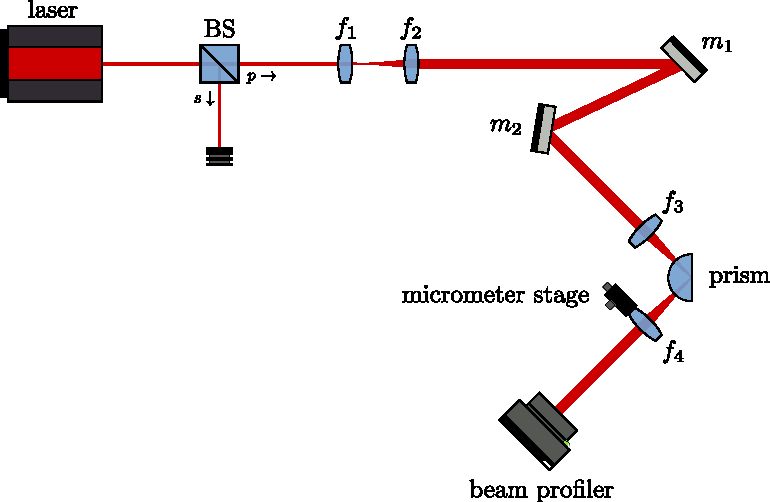
\includegraphics[keepaspectratio,width=14cm]{interference/figures/opticalsetup.pdf}
\caption{Experimental setup.  Light from a laser passes through beamsplitter
BS passing p-polarized light and expanded by two lenses, $f_1$ and $f_2$.
Mirrors $m_1$ and $m_2$ steer the expanded beam to lens $f_3$, focusing the
light on to hypotenuse of a hemispherical prism.  Lens $f_4$ re-images the reflected field to a beam profiler where it is recorded.}
\label{fig:opticalsetup}
\end{figure}
Experimental verification of the predictions of Equations~\ref{eqn:fourier123}
and~\ref{eqn:fourier321} was performed with the setup shown in
\Figure{fig:opticalsetup}.  Light from an
unpolarized \SI{30}{\milli\watt} \SI{632.8}{\nano\meter} helium-neon
laser first passes through the polarizing
beamsplitter BS\@.  It is then expanded and re-collimated by lenses $f_1$ and $f_2$ as an
approximately Gaussian beam with a $1/\me^2$ beam waist of
\SI{3}{\milli\meter} The light is steered by mirrors $m_1$ and $m_2$ to
lens $f_3$, antireflection coated aspherical lens with a focal length of
\SI{20}{\milli\meter}, which
focuses the light to the central point of the hypotenuse of a
\SI{10}{\milli\meter} diameter LAH79 hemispherical prism
($n(\SI{632.8}{\nano\meter})\approx1.98$).  The beam makes a central angle
of $\thetasp\approx\SI{32}{\degree}$ with the hypotenuse.
On the hypotenuse of the prism is a \SI{49.8}{\nano\meter} silver film
obtained through a sputtering process (See \Section{sec:expsputtering}).
The specific thickness was chosen to
optimizes the far field ATR minimum in the specularly reflected
direction.  Silver was used because it has the longest SPP propagation
length of all readily available sputtering targets.
Consistent with the Fourier optics perspective, a longer SPP propagation
length on the interface results in a narrower resonance linewidth in the
far field and vice versa.  An LAH79 hemispherical prism was used because of
its high refractive index ($n\approx 1.98$ at \SI{632.8}{\nano\meter}) and
because its hemispherical shape permits observation of scattered light with
minor distortion.  The totally internally reflected or scattered light is
optionally imaged at this point by the lens $f_4$, which is identical to
lens $f_3$.  The optical fields are observed by direct projection on a 10-bit
CCD sensor (beam profiler).  Since most of the interesting spatial structure of the
reflected beam occurs in a small spatial range, Lens $f_4$
is mounted on a micrometer stage.  As the stage is translated, different focal
planes can be imaged.

\begin{figure}[ht]
 \centering
 \import{includes/}{setpgfinc}
 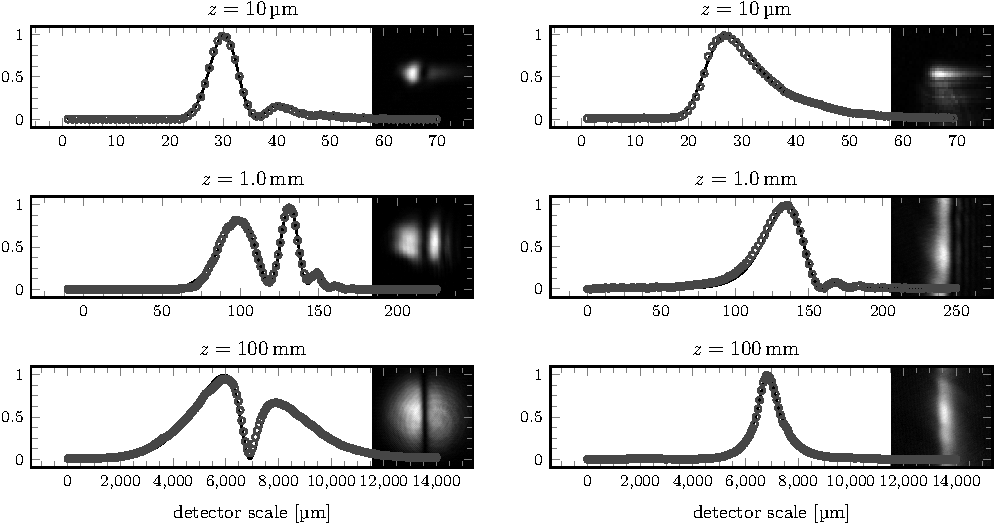
\includegraphics[width=16cm,keepaspectratio]{interference/figures/fig2-crop.pdf}
\caption{Theoretical and experimental values of
$|E_\text{notch}(x,z)|^2$ and $|E_\text{cone}(x,z)|^2$ obtained for three
characteristic propagation distances.  Theoretical values are solid lines,
while experimental values are shown with points.  Distances are
approximate.  Inset is the experimentally obtained optical intensity.}
\label{fig:fresnelprop}
\end{figure}
Verification of the optical fields were obtained using a beam profiler for an
optimally focused lens $f_3$ while the focal plane of lens $f_4$ was moved
normal to the direction of radiation.  Images at increasing distances from the
surface were taken of light in both the notch ($\phi=0$) and the cone at an
angle $\phi = \SI{90}{\degree}$.  Since the cone is more or less radially
isotropic, the choice of $\phi$ in this experiment is arbitrary as long as it
is far enough away from the incident or specular beam.  The data is shown in
\Figure{fig:fresnelprop} along with theoretical calculations based on
Equations~\ref{eqn:fourier123} and~\ref{eqn:fourier321}. Linear (2D) sections
of the experimentally obtained results for three different characteristic
propagation distances are also shown.  The $z=\SI{10}{\micro\meter}$ and
$z=\SI{100}{\milli\meter}$ distances are representative of the near and far
field; their optical fields related by a Fourier transform.  The intermediate
propagation distance $z=\SI{0.1}{\milli\meter}$ was chosen because of the high
visibility of the interference fringes.  As is evident from the figures, as
the field propagates it diffracts, exhibiting an evolving asymmetric
fringe structure between the near and far fields.  The experimentally
obtained field matches well with theoretical calculations using an unmodified
Drude model for silver.

The far field is often defined as as $z\gg 2 D^2/\lambda$, where $D$ is the
spatial width of the source.  For silver at \SI{632.8}{\nano\meter}, the
Lorentz-Drude
model permittivity is $\epsilon = \num{-14.48+1.09i}$ and the $1/\me$ SPP
propagation distance normal to the interface $D = 1/(2 k_x) \approx
\SI{17}{\micro\meter}$ and the resulting far field limit is $2 D^2/\lambda
\approx \SI{10}{\milli\meter}$.  This seems to be consistent with both the
simulated and experimental results, as it is approximately the distance in
\Figure{fig:fresnelprop} for which the interference fringes disappear.

At $z=0$, $|E_\text{notch}(x,z=0)|^2$ matches the near field theoretically
predicted via a similar method by \name{Chuang}~\cite{chuang1986lateral}, or
through vector Gaussian beam decomposition~\cite{baida1999theoretical}, shown
in \Figure{fig:baidacompare} for comparison.  It has also been experimentally
verified through near field optical measurements~\cite{dawson2001surface},
though this only permits observation of the field on the 2--3 interface, or
$|E_\text{cone}(x,z=0)|^2$.  Near field measurements of the 1--2 interface are
not possible due to the presence of the prism.  It is interesting that both
fields have been obtained using optical-only methods; both SPP propagation and
radiative decay are obtained simultaneously.  The results by \name{Baida}
(\Figure{fig:baidacompare}) are very similar to what was obtained in
\Figure{fig:fresnelprop}.  In this sense,
$|E_\text{cone}(x,z=\SI{10}{\micro\meter})|^2$ approximates the field on the
metal-vacuum/air (2--3) interface and
$|E_\text{notch}(x,z=\SI{10}{\micro\meter})|^2$ the metal-glass (1--2)
interface.  The SPP propagation distance is greater for \name{Baida} due to a
difference in the value chosen for the permittivity of silver:
\num{-17.9+0.7i} versus the value of \num{-14.48+1.09i} used for the
calculation of \Figure{fig:fresnelprop}.

\begin{figure}[ht]
\centering
\import{includes/}{setpgfinc}
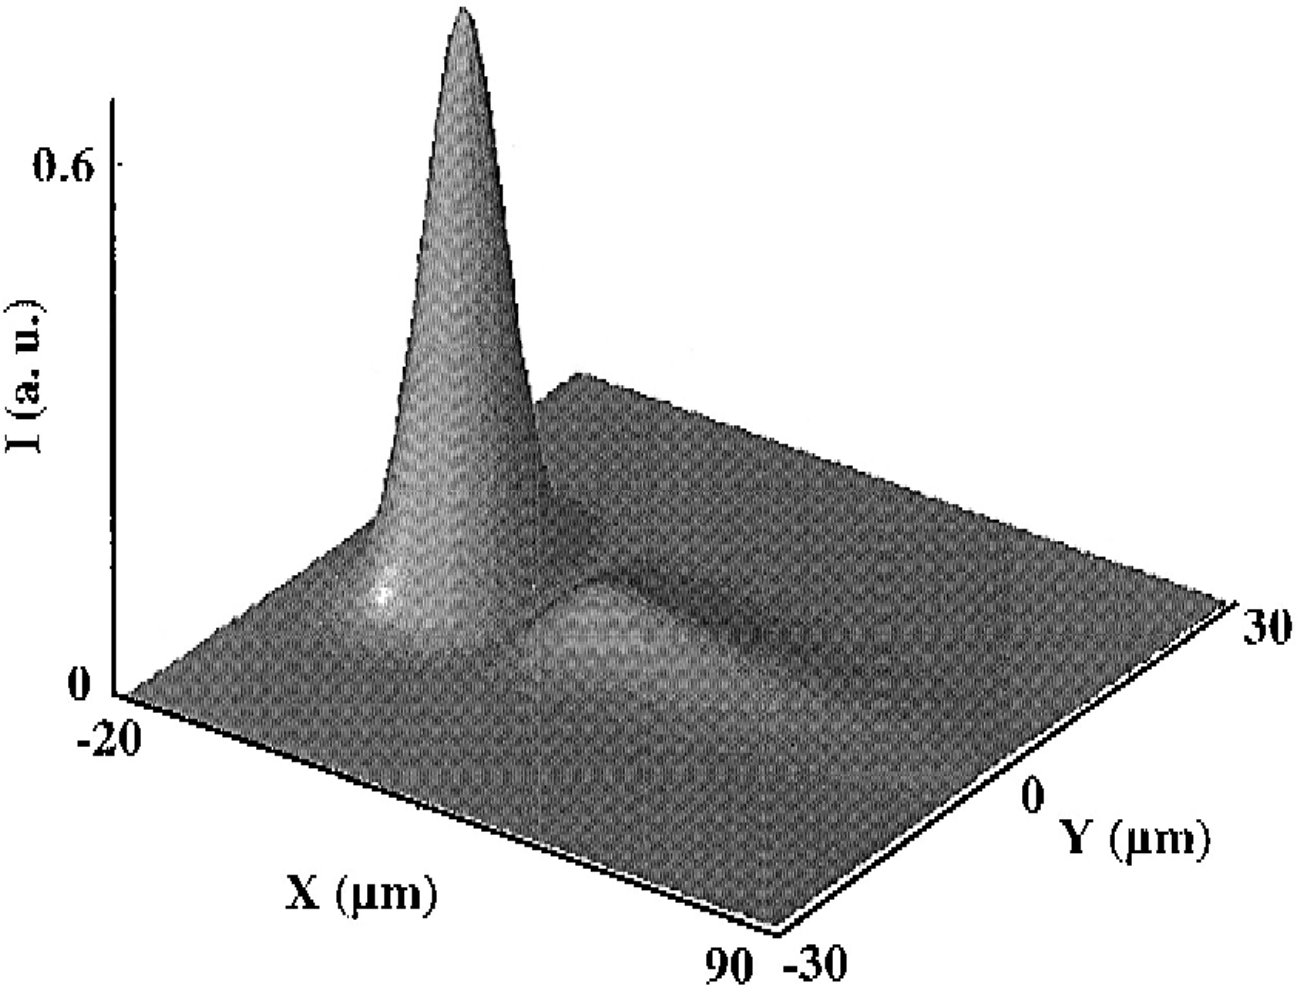
\includegraphics[keepaspectratio,width=6cm]{interference/figures/BaidaReflected.png}
\hspace{1cm}
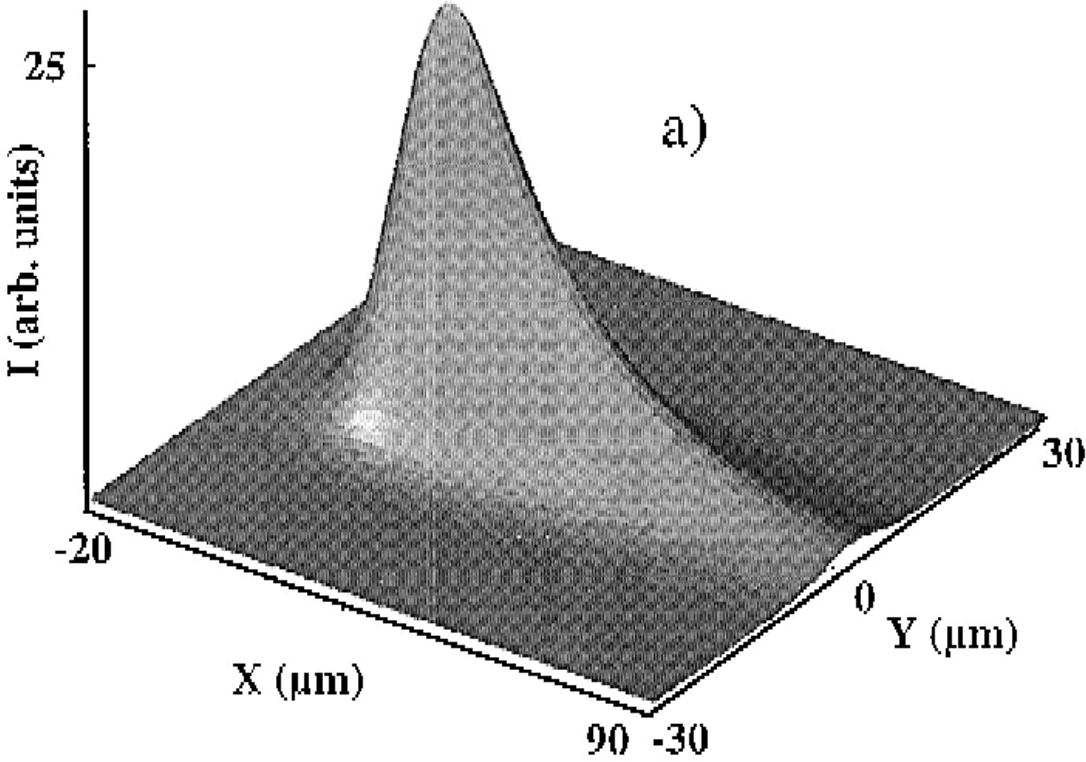
\includegraphics[keepaspectratio,width=6cm]{interference/figures/BaidaTransmitted.png}
\caption{Predictions of the optical field made by
				\name{Baida}~\cite{baida1999theoretical}.  On the left is the field on
				the metal-glass (1--2) interface.  On the right, the field on the
				metal-vacuum (2--3) interface.  Compare with the near fields for the
				notch and cone in \Figure{fig:fresnelprop}.}
\label{fig:baidacompare}
\end{figure}

As a final comparison, \Figure{fig:dawsoncompare} shows a near-field
measurement of the optical field on the metal-air (2--3) surface made by
\name{Dawson}~\cite{dawson2001surface} using a photon scanning tunneling
microscope (PSTM).  As mentioned, this method only permits measurements on one
side of the metal film.  Again, except for the differing values of the
dielectric function for silver (determining the propagation length, see
\Section{sec:sppphysicalchar}), the results match \name{Baida} and 
\Figure{fig:fresnelprop}.
\begin{figure}[ht]
\centering
\import{includes/}{setpgfinc}
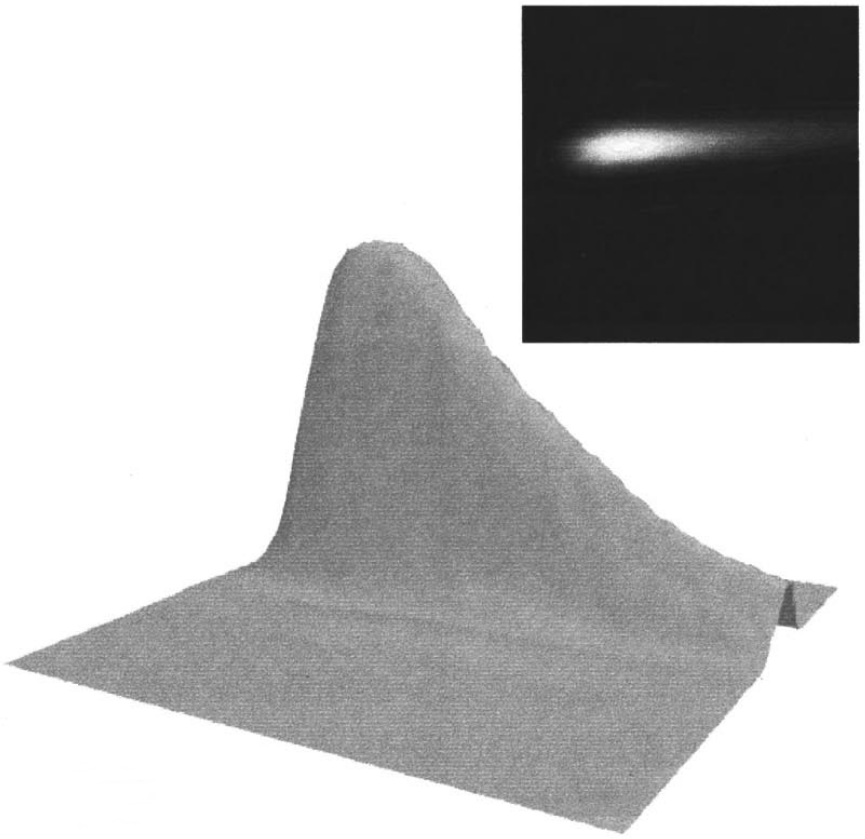
\includegraphics[keepaspectratio,width=6cm]{interference/figures/DawsonTransmitted.png}
\caption{Photon scanning tunneling microscope image of the metal-vacuum (2--3)
				interface from \name{Dawson}~\cite{dawson2001surface}.  No scale was
				given except that the $1/\me$ propagation length was
				\SI{13.8}{\micro\meter}.  Compare with
				the near field cone image in \Figure{fig:fresnelprop}.  The model of
				\name{Dawson} assumes a \SI{2.65}{\nano\meter} layer of \ce{Ag2S} on
				top of the silver layer, hence the reduced SPP propagation length.}
\label{fig:dawsoncompare}
\end{figure}


\subsection{Interference and Diffraction}
Previous reports of the spatial interference fringes in the specular direction
for long range surface plasmons~\cite{simon2007observation} and localized
surface plasmons~\cite{schumann2008near} have described it as arising due to
interference between the specular reflection of the Gaussian beam from the
1--2 interface and the re-radiated plasmon field from the 2--3 interface.
These components can be identified by the two peaks in the near field specular
signal (\Figure{fig:fresnelprop}, $z=\SI{10}{\micro\meter}$).  While it is true that the field in the specular direction contains
both components, and that $\tilde{r}_{12}$ and $\tilde{r}_{23}$ are indeed
antiphase at $k_\text{sp}$ the fringes do not require a specular component to
be observed.
\begin{figure}[ht]
\centering
\import{includes/}{setpgfinc}
\import{interference/figures/}{r123m12}
\caption{Comparison of the propagated $\tilde{r}_{123}(k_x)$ verses
$(\tilde{r}_{123}(k_x)-\tilde{r}_{12})$.  Note that interference fringes occur in
both cases.  }
\label{fig:r123m12}
\end{figure}

In \Figure{fig:r123m12}, the contribution of the 1--2 interface has been
removed by propagating $\tilde{r}_{123}-\tilde{r}_{12}$ to
$z=\SI{1.17}{\milli\meter}$.  Nevertheless, the fringes persist despite the
absence of $\tilde{r}_{12}$.  In terms of the experiment, removing
$\tilde{r}_{12}$, the specular reflection, is equivalent to what is found in
the cone (itself containing fringes).

In light of these observations, it is more correct to ascribe the fringe
structure as being a diffraction, rather than a two component interference
phenomena motivated by phase alone (although there are two components in the
specular direction).  Note that similar behavior is found in almost any causal
function propagated by a free space transfer term, for example the Fourier
transformed Lorentzian absorption $\tilde{f}(k) = 1/(1+\mi k)$.

The asymmetry of the interference results from the causality of the system.
Assume a complex function $\chi(\omega) = \chi'(\omega) + \mi \chi''(\omega)$
whose real and imaginary parts are related by Kramers-Kronig relations
\begin{align}
\chi(\omega)=\mi \hf{\chi(\omega)}
\end{align}
with 
\begin{align}
\chi'(\omega) &= \hf{\chi''(\omega)}\\
\chi''(\omega) &= -\hf{\chi'(\omega)}
\end{align}
where $\hf{\chi(\omega)}$ is the Hilbert transform of $\chi(\omega)$.
The Fourier transform of $\chi(\omega)$ is
\begin{align}
\chi(\omega) &= \chi'(\omega) + \mi \chi''(\omega)\\
\ff{\chi(\omega)} &= \ff{\chi'(\omega) + \mi \chi''(\omega)}\\
&= \ff{\chi'(\omega)} + \ff{\mi \chi''(\omega)}\\
&= \ff{\chi'(\omega)} + \ff{\mi \hf{\chi'(\omega)}} \\
&= \ff{\chi'(\omega)} + \sgn(\omega) \ff{\chi'(\omega)} \\
\end{align}
Or succinctly,
\begin{align}
\ff{\hf{\chi(\omega)}} = (-\mi \sgn(\omega)) \ff{\chi(\omega)}
\end{align}
In other words, the Fourier transform of any function which satisfies
Kramers-Kronig relations is asymmetric (``one-sided'') as a necessary
condition of causality.  This condition is also known as Gibb's phenomena.
Since no physical system can respond infinitely fast to an input signal, high
frequency components are lost.  In the case of SPR occurring at the focus of
an incident Gaussian beam, it can be seen as a spatial filter which modifies
the local $k$-vectors to produce the resulting far field optical pattern.  If
the SPR resonance condition is sharp, the Fourier integral
(\Equation{eqn:fourier123}) is truncated and the plasmon resonance acts as a low
pass filter for light.  
